
\section*{Context}
Networks are objects representing relationships between entities. They are useful to comprehend systems joint organization and behaviors, leading to discoveries that would not have been possible by analyzing the entities separately. Applications are numerous in life sciences, among which genes regulatory networks (genomics), community assembly mechanisms (community ecology), or pathobiome organization (microbiology). Networks can be built from observed interactions, as is the case of host-parasite, plant-pollinator or trophic networks in ecology, or protein-protein interaction networks in genomics. However this strategy, which we call network reconstruction, limits the identified interactions to observable ones only, where others would be interesting too (e.g. competition for food or space, shelter sharing, etc.).\\

 
\begin{figure}[H]
\centering
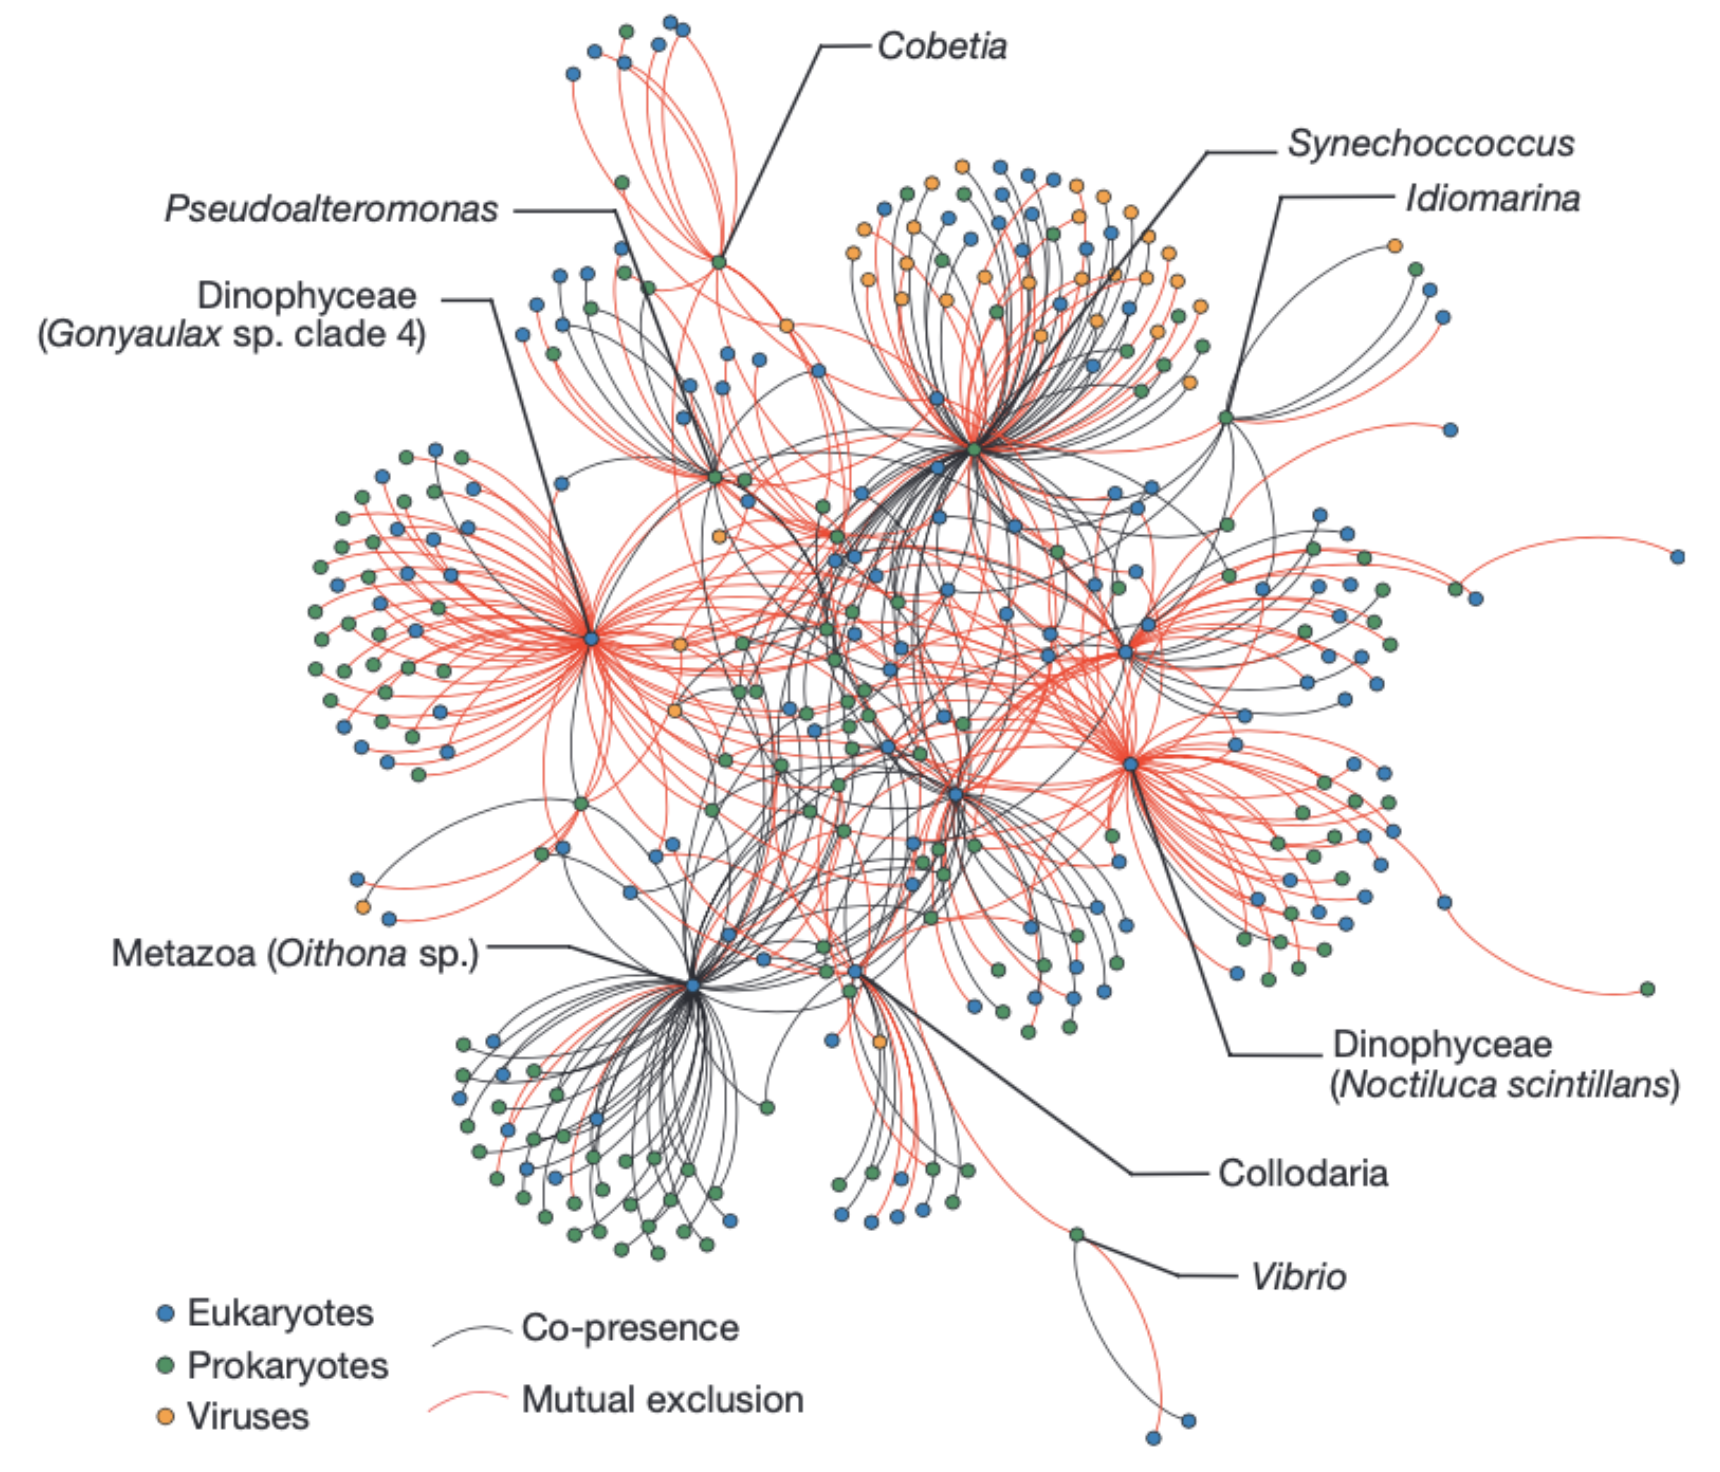
\includegraphics[width=0.7\linewidth]{figs/plancton.png}
\captionsetup{labelformat=empty}
\caption{Integrated plankton community network related to carbon export at 150m \citep{GCB16}.}
\label{PPI}
\end{figure}



This work is interested in species network inference, which is the art of identifying interactions from observed measures on a set of species. Network inference necessarily relies on a mathematical definition of species interactions, allowing to detect a broad range of interactions. Their biological meaning is unknown and would have to be identified by experts later on. 


A first idea of a mathematical species interaction is the correlation between the species abundances. However using correlation results in dense networks proving hard to analyze, as spurious edges appear between two variables correlated to the same third one \footnote{e.g. the number of covid 19 cases detected correlates with both the real number of cases and the number of tests done on the population, which induces a spurious correlation between the two latter where obviously there is no direct effect of one on the other.}.  Instead, using conditional dependence relationships between species provides with  a clear separation between direct and indirect effects, and therefore yields sparse and easy to interpret networks.


Graphical models are the dedicated mathematical framework for the modeling and inference of such networks, for they graphically represent a multivariate random variable conditional dependencies. Gaussian Graphical Models (GGM) in particular present with specific theoretical and algebraic properties which facilitate the inference. GGM  have been widely used on continuous data. \\

However measures on species are often counts, as is usually the case in ecology and in experiments using high-throughput sequencing technologies in genomics and microbiology. A way to go for network inference from count data with a distinction between direct and indirect effects is then to adopt a modeling for the count allowing the use of the GGM framework. To obtain interpretable results, the model should also account for measured experimental offsets and covariates. Furthermore, the observed measures on species are also very likely to be incomplete as it is difficult to know in advance all the factors governing a phenomenon. This causes the species interaction network to present spurious edges between the species which should be linked to the unobserved actor (species or covariate). A partial observation of the data thus provides with a marginal network instead of the complete one, leading to biased further interpretations and analyzes.\\


\section*{Objectives and outline} 
The aim of the present work is to develop a methodology for the network inference from incomplete abundance data. This task was divided into two sub-objectives. 
First, develop a method for network inference from abundance data. To this aim we model counts  using the Poisson log-normal distribution, taking advantage of the estimation procedure developed by \citet{CMR18}. This specific distribution includes a latent layer of Gaussian parameters, within which the inference of the species interaction network is performed. Following \citet{MeilaJaak} and \citet{SR17}, the inference is carried out using tree averaging, allowing for a complete and efficient exploration of the space of spanning tree graphs, and yielding edges probabilities.

Then, this work includes missing actors in the model to account for incomplete data. There we model the missing actors as additional latent variables of the model Gaussian latent layer. The Gaussian graphical model parameters maximum likelihood estimators detailed in \citet{Lau96} are adapted to the specific case of spanning tree structures, and applied within a variational Expectation Maximization algorithm.

  \subsection*{Chapter 1}
The first chapter covers in details the mathematical and technical background used in Chapters 2 and 3. It defines the general framework of graphical models and its link with conditional independence relationships. The particular properties of the Gaussian graphical models are then presented, along with its maximum likelihood estimators. Two network inference methods are detailed: the penalized regularization which estimates the precision matrix in a sparse manner, and tree averaging which efficiently explores the super-exponential space of spanning-tree structures. This chapter then draws a state of the art of the strategies for the modelization of multivariate counts.

   \subsection*{Chapter 2}
   Chapter 2 details the proposed methodology for the inference of species interaction networks from measures of joint abundances. Counts are modeled in a hierarchical manner: a spanning-tree graph $T$ is first drawn, then parameters $\Zbf$ are modeled  conditionally on $T$ as a multivariate Gaussian faithful to $T$, and finally counts $\Ybf$ follow a Poisson log-normal distribution with parameters $\Zbf$. This model thus involves two latent layers of parameters: $\Zbf$ and $T$, and can be described by the following graph:
 
 \begin{center}
	\begin{tikzpicture}	
      \tikzstyle{every edge}=[-,>=stealth',auto,thin,draw]
		\node (A1) at (0*\length, 0*\length) {$T$};
		\node (A2) at (1*\length, 0*\length) {$\Zbf$};
		\node (A3) at (2*\length, 0*\length) {$\Ybf$};
		\draw (A1) edge [->](A2);
        \draw (A2) edge [->] (A3);
	\end{tikzpicture} 
   \end{center}
 
The model inference estimates the tree distribution using an EM algorithm, which had not been done before. The proposed methodology is implemented in the R package EMtree (\url{github.com/Rmomal/EMtree}). It is compared to state-of-the-art approaches and applied to two empirical datasets from ecology and microbiology. This chapter has been published in the journal \textit{Methods in Ecology and Evolution} \citep{MRA20}. The presented appendices are extended with a vignette showing usage examples of the EMtree package.

    \subsection*{Chapter 3}
This chapter presents an extended version of the previous model developed in Chapter 2 to include possible missing actors. The Gaussian latent layer is assumed to involve additional unobserved variables. The Gaussian layer is considered in its normalized form and denoted $\Ubf$.  This model thus involves three latent layers: $T$, $\Ubf_O$ where "O" stands for "observed", and $\Ubf_H$ where "H" stands for "hidden", and can be described by the following graph:
 
 \begin{center}
	\begin{tikzpicture}	
      \tikzstyle{every edge}=[-,>=stealth',auto,thin,draw]
		\node (A1) at (0.625*\length, 2*\length) {$T$};
		\node (A2) at (0*\length, 1*\length) {$\Ubf_O$};
		\node (A3) at (1.25*\length, 1*\length) {$\Ubf_H   $};
		\node (A4) at (0*\length, 0*\length) {$\Ybf$};
		\draw (A1) edge [->](A2);
        \draw (A1) edge [->] (A3);
        \draw (A2) edge  (A3);
        \draw (A2) edge [->](A4);
	\end{tikzpicture} 
	  \end{center}
 
 The model is estimated with a variational EM algorithm, which takes advantage of the average on trees to use the adaptation to the context of spanning trees of the maximum likelihood estimators of GGM parameters detailed in \citet{Lau96}. The developed procedure is implemented in the R package nestor (\url{github.com/Rmomal/nestor}) and illustrated on two  empirical datasets from ecology. \\

This chapter has been submitted for publication in a statistical journal. The submitted supplementary material is enriched with a vignette showing usage examples of nestor, a section presenting different initialization methods and finally a comparison of nestor, EMtree and  PLN-network which is another method building on the PLN distribution but uses a penalized approach for the network inference.

  \subsection*{Chapter 4}
This final chapter introduces some perspectives of this work. After summarizing  the specifics of the developed methodology and discussing unresolved issues, natural extensions of the model are presented. They first include extensions about measures on the inferred network, with a method for estimating the latent layer precision matrix,  and a strategy  to use tree distributions for comparing networks. Then perspectives about the data at hand are discussed, namely how to handle other data types or datasets presenting with spatial dependencies. Finally a model for the network inference not resorting to a latent layer is presented. %using only discrete distributions is presented.
\newpage
 \section*{Notations}
 
 \begin{description}
 \item[Operations:]  \begin{itemize}
     \item[]
 \item[] $|\cdot|$ : matrix determinant
 \item[] $\odot$ : Hadamard product
 \end{itemize}
 \item[Matrices:] \begin{itemize}
     \item[]
 \item[] $\Ybf$ : observed counts
 \item[] $\Zbf$ :  latent Gaussian parameters 
 \item[] $\Ubf$ :  latent normalized Gaussian parameters 
 \item[] $\Xbf$ : covariates 
 \item[] $O$ :  measured offsets
 \end{itemize}
 \item[Dimensions:]\begin{itemize}
     \item[]
 \item[] $n$ : samples
 \item[] $p$ : observed species
 \item[] $r$ : unobserved actors
 \item[] $d$ : covariates
 \end{itemize}
 \end{description} 